\section{Bézier Curves}
First we will go over some preliminaries that are useful to know before we get to actual Bézier curves. Then we introduce the general concept of Bézier curves and give an overview how we implemented the different methods to calculate Bézier curves followed by detailed sections about these methods and their implementation.
\subsection{Linear Interpolation}
\begin{definition}(Straight Line)
Let $a, b \in \mathbb{R}^2$ be 2 points. A \textbf{straight line} is defined as the set of all possible combinations
\[x = x(t) = (1-t) \cdot a + t \cdot b\]
where $t \in [0,1]$.
\end{definition}
But we can also express $t$ as $t=(1-t) \cdot 0 + t \cdot 1$. Hence $t$ is also just a point lying on a straight line between $0$ and $1$ and therefore the points $a,x,b$ are an \textbf{affine map} on $0,t,1$.
\begin{definition}(Linear Interpoaltion)
\textbf{Linear interpolation} is an affine map of the real line onto a straight line.
\end{definition}
Since we see linear interpolation as an affine map we get the following property.
\begin{definition}
Linear interpolation is \textbf{affine invariant}. Thus the following holds
\[\phi(x) = \phi((1-t) \cdot a + t \cdot b) = (1-t) \cdot \phi(a) + t \cdot \phi(b)\]
where $\phi$ is an affine map, $t \in [0,1]$ and $a,b$ are two points in $\mathbb{R}^2$.
\end{definition}


\subsection{Piecewise Linear Interpolation}
% Mein Vorschlag
\begin{definition}(Polygon)
A \textbf{Polygon} is defined as a finite sequence of points $b_0,\dots,b_n \in \mathbb{R}^m$ where each two consecutive points $b_i$ and $b_{i+1}$ are connected by a straight line.\\
\end{definition}
With this we can define the piecewise linear interpolant of a curve $c$.
\begin{definition}(piecewise linear interpolant)
Let $c$ be a curve. The polygon interpolating the $b_i$ is the \textbf{piecewise linear interpolant} $PL$ of $c$ if and only if all points lie on $c$.
\end{definition}
\begin{rem}
One can easily show that the piecewise linear interpolant is \textbf{affinely invariant}, which means that for any curve $c$ and affine map $\phi$
\[
PL(\phi(c)) = \phi(PL(c))
\]
\end{rem}


\subsection{Menelaos' Theorem}
\begin{theorem}\label{Men}
Let $b$ be an open polygonal chain of $b_0, b_1, b_2 \in \mathbb{R}^2$.  We can define any points on the straight lines as convex combinations of those points.
\begin{align*}
    b[0,t] &= (1-t) \cdot b_0 + t \cdot b_1\\
    b[s,0] &= (1-s) \cdot b_0 + s \cdot b_1\\
    b[t,1] &= (1-t) \cdot b_1 + t \cdot b_2\\
    b[s,1] &= (1-s) \cdot b_1 + s \cdot b_2\\
\end{align*}
Where $s,t \in [0,1]$ and $b[*, *]$ is a two-dimensional blossom (we will talk more about blossoms in the next section). With this we define $b[s,t], ~ b[t,s]$ as:
\begin{align*}
    b[s,t] &= (1-t) \cdot b[s,0] + t \cdot b[s,1]\\
    b[t,s] &= (1-s) \cdot b[0,t] + s \cdot b[t,1]
\end{align*}
Menelaos' theorem now simply states
\[
    b[s,t] = b[t,s]
\]
\end{theorem}
\begin{proof}
\begin{align*}
    b[s,t] &= (1-t) \cdot b[s,0] + t \cdot b[s,1]\\
    &= (1-t) \cdot ( (1-s) \cdot b_0 + s \cdot b_1 ) + t \cdot ( (1-s) \cdot b_1 + s \cdot b_2 ) \\
    &= (1-t) \cdot (1-s) \cdot b_0 + (1-t) \cdot s \cdot b_1 + t\cdot (1-s) \cdot b_1 + t \cdot s \cdot b_2\\
    &= (1-t) \cdot (1-s) \cdot b_0 + t\cdot (1-s) \cdot b_1 +  (1-t) \cdot s \cdot b_1 +t \cdot s \cdot b_2\\
    &= (1-s) \cdot ( (1-t) \cdot b_0 + t \cdot b_1 ) + s \cdot ( (1-t) \cdot b_1 + t \cdot b_2 )\\
    &= (1-s) \cdot b[0,t] + s \cdot b[t,1]\\
    &= b[t,s]
\end{align*}
\end{proof}
This means that the resulting point is continuous linear interpolation is invariant to the order of weights used.
\begin{figure}[H]
    \centering
    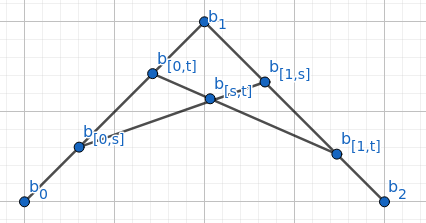
\includegraphics[width=15em]{Menelaos3.png}
    \caption{Points defined on the straight line of our previously defined points}
    \label{fig:Men}
\end{figure}
\subsection{Blossoming}
\begin{definition}(Blossoms)
\textbf{Blossoms} are a multivariate function. Denoted $b[t_1, \dots, t_n]$, where $t_i \in \mathbb{R}$ for $i \in \{1, \dots, n\}$. 
\end{definition}
So in each interpolation step a different $t$ can be used.
Blossoms have some very interesting properties that are useful for types of Bézier curves:
\begin{lem}\label{sym}(\textbf{Symmetry})
In the case of Blossoms the order of the arguments does not change anything; in fact this is an application of \cref{Men}:
\[b[t_1, \dots, t_n] = b[\pi(t_1, \dots, t_n)]\]
where $\pi(t_1, \dots, t_n)$ denotes some permutation matrix and $t_i \in \mathbb{R}$ for $i \in \{1, \dots, n\}$.
\end{lem}
Before we can look at the next property let us fist define \textbf{Multi Affinity} and \textbf{barycentric combinations}.
First we will define multi affinity.
\begin{definition}(Multi Affinity)
A function is \textbf{multi affine} if it is affine in regards to every parameter.
\end{definition}
Now let us introduce barycentric combinations.
\begin{definition}
Let $P_1, \dots, P_n$ be points in $\mathbb{R}^m$ and $\alpha_1, \dots, \alpha_n$ be weights in $\mathbb{R}$.
A \textbf{barycentric combination} of the points $P_1, \dots P_n$ is a weighted sum\[\sum_{i=1}^n \alpha_i \cdot P_i\] with the affinity constraint
\[\sum_{i=1}^n \alpha_i = 1\]
\end{definition}
 Before we look at the general case, let us examine a simple example:
\[b[\alpha \cdot r + \beta \cdot s, t_2] = \alpha \cdot b[r, t_2] + \beta \cdot b[s, t_2]\]
So if the first argument is a barycentric combination, we can compute the blossom values separately and then build the barycentric combination. Of course we are not restricted to the case for the first argument, since we have symmetry. In general we have:
\begin{lem}(\textbf{Multi Affinity})
\[b[\alpha \cdot r + \beta \cdot s, *] = \alpha \cdot b[r, *] + \beta \cdot b[s, *]\]
where $\alpha + \beta = 1$, $r,s \in \mathbb{R}$ and $*$ denotes the same arguments. However the order of the parameters does not play a role, as shown in \cref{sym}.
\end{lem}
\begin{rem}(\textbf{Diagonality})
Let $t = t_1 = \dots = t_n$ and $t_i \in \mathbb{R}$ for $i \in \{1, \dots, n\}$. In this case we obtain a polynomial curve or Bézier curve. We use the notation:
\[b[t, \dots, t] = b[t^n]\]
if the argument $t$ is repeated $n$ times.
\end{rem}
\newpage
\subsubsection{Leibniz Formula}
If we use the properties we just defined we can consider a special case where we have $(\alpha \cdot r + \beta \cdot s)$ $n$ times as argument. We get:
\begin{lem}\label{leib}(\textbf{Leibniz Formula)}
\[b[(\alpha \cdot r + \beta \cdot s)^n] = \sum_{i=0}^n \binom{n}{i} \alpha^{i} \cdot \beta^{n-i} \cdot b[r^{i}, s^{n-i}]\]
\end{lem}
\subsection{Definition of Bézier Curves}
Before we will have a look at different types of Bézier Curves and how they can be calculated. Let us first define what a Bézier Curve is.
\begin{definition}
A \textbf{Bézier curve} is a parametric curve described by control points $b_0, \dots, b_n \in \mathbb{R}^2$. These points form the so called Bézier polygon or control polygon the $b_i$ are called \textbf{Bézier points} or \textbf{control points}, and we use these terms interchangeably. The degree of the curve described by the polygons is $n-1$. \\
\end{definition}
The actual Bézier curve can be formed using a variety of different formulas that all use some weight $t$, which is normally on the unit interval, on the Bézier points. So we write $b_0^n(t)$ for an actual point on the curve and $b_i^0(t) := b_i$ for the Bézier points, similar to the notion we already used in the blossom section.

\begin{figure}[H]
    \centering
    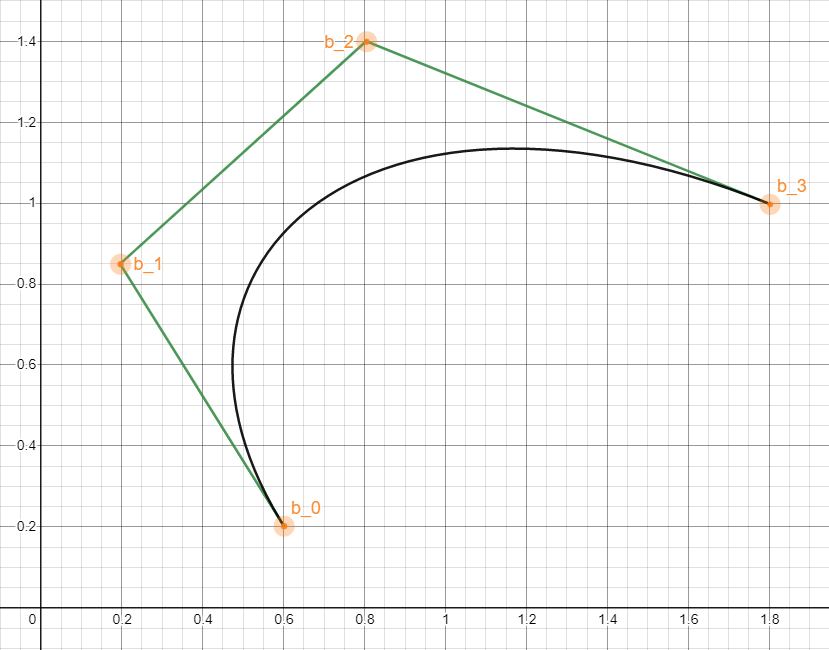
\includegraphics[width=0.7\textwidth]{Beispiel_Bezierkurve.png}
    \caption{Example Bézier curve with control polygon}
    \label{fig:my_label}
\end{figure}

\subsection{General Implementation of Types of Bézier Curves}
To implement the different types of Bézier curves we use a clever class hierarchy. \\

% picture here
We use an abstract class as our base. This one implements most of the methods all of its children use. Like the derivative, addition, multiplication and so on. \\

The most fundamental function is the curve function, which is a cached property. Calling this method generates the preferred amount of evaluated points for the given Bézier points. The curve function supports either parallel or serial execution.\\

The curve is based on the abstract \texttt{init\_func}, which is the only method that needs to be provided by any subclass. This makes inheritance very elegant.

\begin{figure}[H]
    \centering
    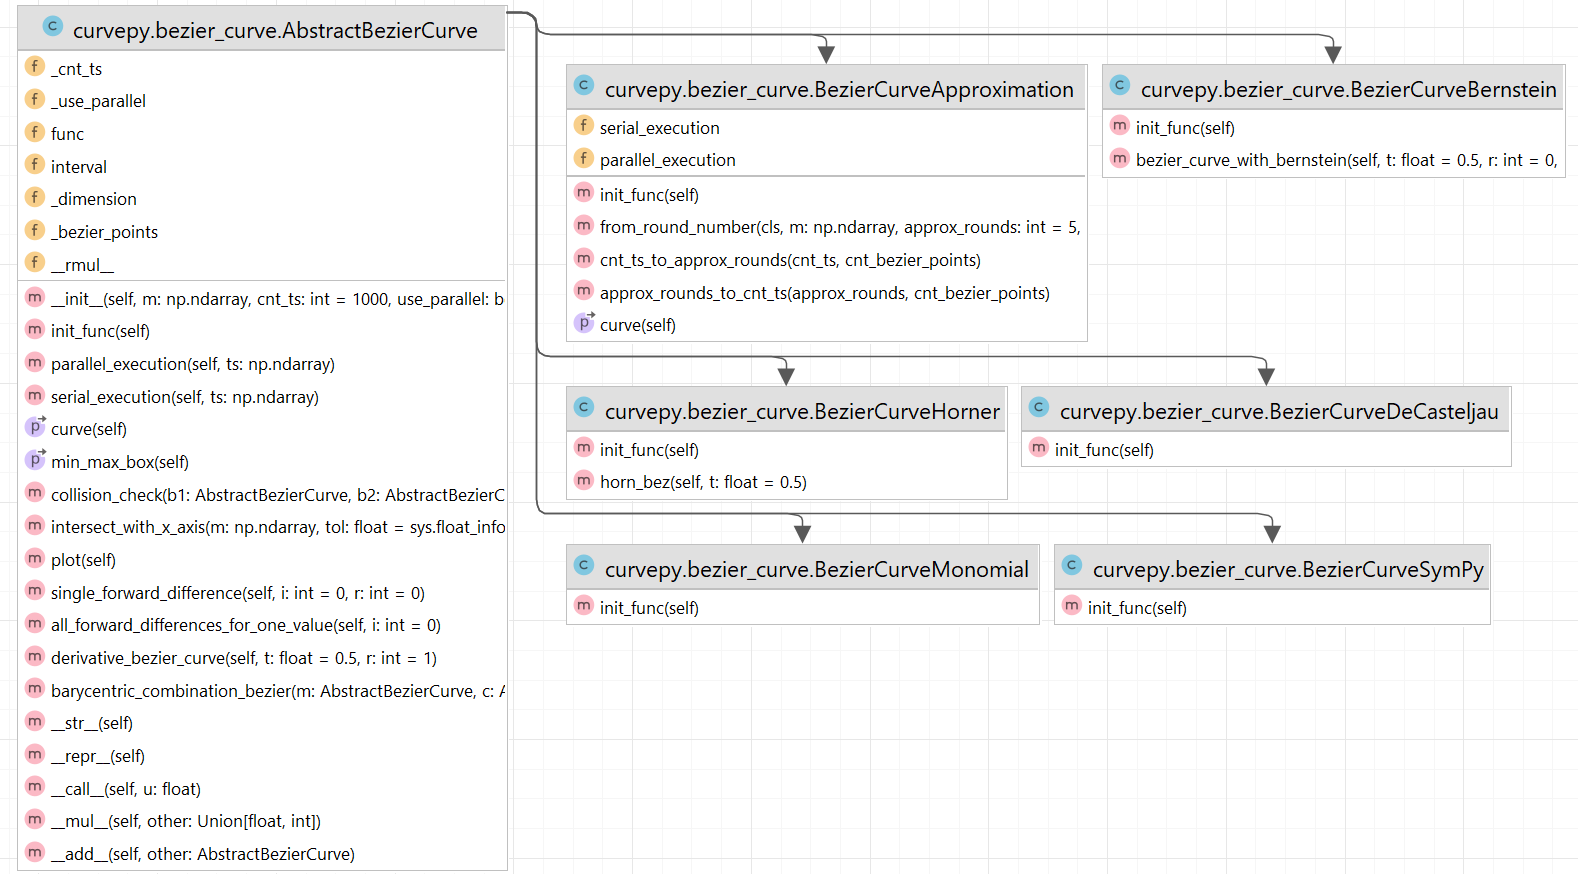
\includegraphics[width=\textwidth]{uml.png}
    \caption{UML class diagram of all Bézier curves}
    \label{fig:my_label}
\end{figure}
\newpage
\subsection{De-Casteljau Algorithm}
In this section we will first introduce the De-Casteljau algorithm which can calculate points lying on a Bézier curve. Following that we explain some interesting properties of Bézier curves and then present our different implementations.

\begin{definition}
Let $b_0, \dots, b_n \in \mathbb{R}^2$ and $t \in \mathbb{R}$, then the following formula is used for the \textbf{De-Casteljau} algorithm:
\[b_i^r(t) = (1-t) \cdot b_i^{r-1}(t) + t \cdot b_{i+1}^{r-1}(t)\]
for $r = 1, \dots, n$ and $i = 0, \dots, n-r$. \\
\end{definition}
\subsubsection{Endpoint Interpolation}
If $t$ is set to $0$ we get $b_0$ (i.e. the beginning) and if it is set to $1$ we get $b_n$ (i.e. the end), which allows for easier usage, especially in design-oriented problems. This is also very handy for composing Bézier curves.

\subsubsection{Invariance under Affine Maps}
Bézier curves are invariant under affine maps, which follows from the De-Casteljau algorithm, since it uses repeated linear interpolation, which is invariant under affine maps. This property is quite handy. For instance if we have four control points and want to evaluate 100 points on the curve described by them and additionally we want to rotate these points, we can just rotate the control points and then compute the 100 points instead of first computing all 100 points and then rotating everyone of them.

\subsubsection{Parameter Transformation}
Another interesting property is that the curve is blind to the actual interval, that the curve is defined over. This is possible, because the algorithm works on ratios. Furthermore we can map a parameter $u$ from an arbitrarily chosen interval $[a,b]$ on our unit interval $[0,1]$ by applying the following transformation: \[t = \frac{u-1}{b-a}\]

\subsubsection{Blossoms and De-Casteljau}
The concept of blossoming can also be used in the De-Casteljau algorithm. One can use a new parameter value $t \in [0,1]$ in each step of the algorithm. Looking at the cubic case we obtain:
\begin{center}
  \begin{tabular}{ l c r r}
  $b_0$ &         \\
  $b_1$ & $b_0^1[t_1]$ &      \\
  $b_2$ & $b_1^1[t_1]$ & $b_0^2[t_1, t_2]$    \\
  $b_3$ & $b_2^1[t_1]$ & $b_1^2[t_1, t_2]$ & $b_0^3[t_1, t_2, t_3]$\\
\end{tabular}
\\
\end{center}
This traces out a region because we use in each of our $r$ steps a different value $t_r$, to recover the original point on the curve we need to set $t = t_1 = t_2 = t_3$ and compute again. 

\subsubsection{Implementation}
We divided the De-Casteljau algorithm in three methods:
\begin{enumerate}
    \item[1] \texttt{de\_casteljau\_one\_step}. This method computes one step of the De-Casteljau algorithm using the following formula:
    \[b_i^r(t) = (1-t) \cdot b_i^{r-1}(t) + t \cdot b_{i+1}^{r-1}(t)\]
    Because of numpy arrays the implementation is straightforward. We utilise slicing and element wise operations on numpy arrays to compute one step without the use of a loop. Additionally we perform most of the heavy work in C++, which makes our implementation significantly faster than only using Python.
    \item[2] \texttt{de\_casteljau\_n\_steps}. This method calls (1) $n$ times, where $n$ lies between \texttt{0} and number of control points minus one and is given by the user. So one can calculate intermediate points or resume calculation from intermediate points.
    \item[3] \texttt{de\_casteljau}: This method computes $b_0^n(t)$ by calling (2) with the proper value for $n$, which is the number of control points minus one.
\end{enumerate}
One drawback is, that we have to explicitly copy the array in certain steps to avoid mistakes, since all python objects, including numpy arrays, are called by reference. We also implemented a parallel version of (3). \\

\begin{figure}[H]
    \centering
    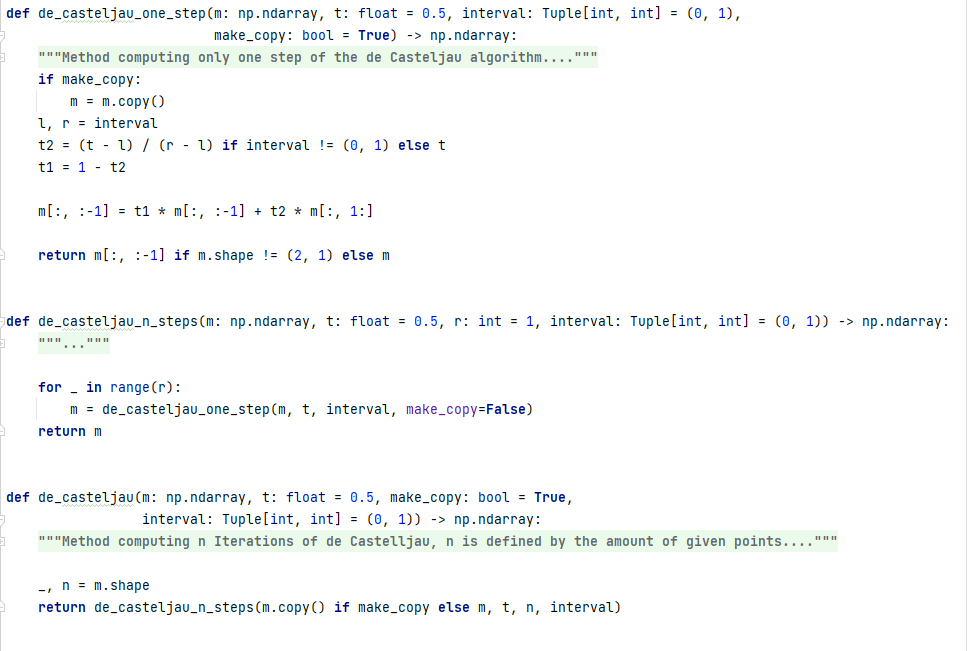
\includegraphics[width=\textwidth]{de_cas.png}
    \caption{De-Casteljau Code}
    \label{fig:my_label}
\end{figure}

There is also a sympy version of the De-Casteljau algorithm, which handels $t$ as a symbolic variable and computes the algorithm without knowing a specific value for $t$, hence we end up with a function representing our curve. At the end we use the lambdify routine to transform our symbolic function to a lambda function, so that we can calculate numerical values faster. Thus for every value of $t$ we just evaluate our lambda function for this value. Sadly, this implementation is limited by the maximum recursion depth allowed by Python.\\

Our blossoming method calls \texttt{de\_casteljau\_one\_step} for different values of $t$ which are defined by the user in a given list.
\newpage
\subsection{Bernstein}
Another way to calculate Bézier curves is to use Bernstein polynomials.
We define them as follows.
\begin{definition}
For $t \in \mathbb{R}$ we define:
\[B_i^n(t) = \binom{n}{i} \cdot t^{i} \cdot (1-t)^{n-i}\]
as the \textbf{Bernstein Polynomial} with parameter $t$, where
\[
\binom{n}{i} =
\left\{
	\begin{array}{ll}
		\frac{n!}{i! \cdot (n-i)!}  & \mbox{: } 0 \leq i \leq n \\
		 0 & \mbox{: } otherwise
	\end{array}
\right.\]
\end{definition}
There is also a recursive formula for Bernstein polynomials:
\begin{definition}
The \textbf{Bernstein polynomial} with parameter $t$ is defined as follows:
\[B_i^n(t) = (1-t) \cdot B_i^{n-i}(t) + t \cdot B_{i-1}^{n-1}(t)\]
where $B_0^0(t)=1$ and $B_j^n(t)=0$ for $j \notin \{0, \dots, n\}$.\\
\end{definition}
We implemented both the recursive and the iterative variant.
\begin{rem}
From the blossoming section we know that we can write Bézier curve as $b[t^n]$, moreover $t$ can be expressed as $t=(1-t) \cdot 0 + t \cdot 1$. By applying \cref{leib} we get
\[b(t) = b[t^n] = \sum_{i=0}^n b_i \cdot B_i^n(t)\]
since $b_i = b[0^{n-i}, 1^{i}]$.
\end{rem}
This results in the following remark:
\begin{rem}
We can express the intermediate points $b_i^r$ in the form of Bernstein polynomials of degree $r$:
\[b_i^r = \sum_{j=0}^r b_{i+j} \cdot B_j^r(t)\]
This follows because of $b_i^r(t) = b[0^{n-r-i}, t^r, 1^{i}]$ and \cref{leib}.
\end{rem}

With this at our hands we get:
\begin{theorem}
Given control points $b_0, \dots, b_n \in \mathbb{R}^2$ and a parameter $t \in [0,1]$. Further let $b_i^r, i \in \{1, \dots, n\}, r < n$ be precomputed. Then we can extend our $b^r$ values as follows:
\[b^n(t) = \sum_{i=0}^{n-r} b_i^r(t) \cdot B_i^{n-r}(t)\]
\end{theorem}

This means that $r$ semantically describes the highest degree of the previously computed Bézier polygon. Thus $r=0$ if and only if no precomputation was made beforehand.\\

Additionally we have the property of invariance under barycentric combinations:
\[\sum_{i=0}^n (\alpha \cdot b_i + \beta \cdot c_i) \cdot B_i^n(t) = \sum_{i=0}^n \alpha \cdot b_i \cdot B_i^n(t) + \sum_{i=0}^n \beta \cdot c_i \cdot B_i^n(t)\]

Therefore we implemented two magic methods namely the \texttt{\_\_add\_\_} and \texttt{\_\_mul\_\_} function. \texttt{\_\_add\_\_} just adds up the given Bézier points of both curves and \texttt{\_\_mul\_\_} multiplies all control points by a scalar value.

\begin{figure}[H]
    \centering
    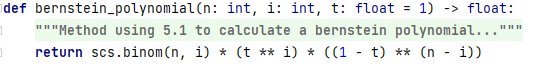
\includegraphics[width=\textwidth]{bernstein_polynomial.png}
    \caption{Bernstein Polynomial Code}
    \label{fig:my_label}
    \centering
    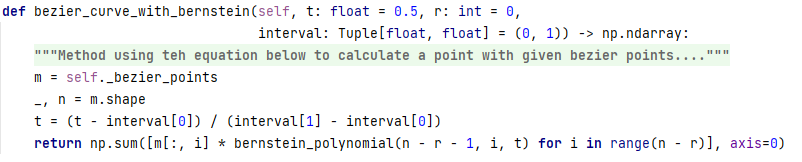
\includegraphics[width=\textwidth]{bernstein.png}
    \caption{Bézier with Bernstein Code}
    \label{fig:my_label}
\end{figure}
\newpage
\subsection{Horner Scheme}
We can also develop an Horner Scheme for the Bézier curves. First we will look at a cubic example.
\begin{example}
\[c_0 + t \cdot c_1 + t^2 \cdot c_2 + t^3 \cdot c_3 = c_0 + t \cdot (c_1 + t \cdot (c_2 + t \cdot c_3))\]

This is the case for a normal polygon on the monomial base, where $c_0, \dots, c_4 \in \mathbb{R}$ and $t \in \mathbb{R}$. We can transform this to Bézier curves and get
\[b^3(t) = \left(\left(\binom{3}{0} \cdot s \cdot b_0 + \binom{3}{1} \cdot t \cdot b_1\right) \cdot s + \binom{3}{2} \cdot t^2 \cdot b_2\right) \cdot s + \binom{3}{3} \cdot t^3 \cdot b_3\]
where $s = (1-t)$, with $t \in \mathbb{R}$ and $b_0, \dots, b_3 \in \mathbb{R}^2$.
\end{example}
Now we can generalize this in the following way:
\begin{definition}
Given $n \in \mathbb{N}$ points $b_0, \dots, b_n \in \mathbb{R}^2$ and a parameter $t \in \mathbb{R}$ we can describe $b^n(t)$ in the following way:
\[b^n(t) = \left(\dots\left(\left(\left(\binom{n}{0} \cdot s \cdot b_0 + \binom{n}{1} \cdot t \cdot b_1\right) \cdot s + \binom{n}{2} \cdot t^2 \cdot b_2\right) \cdot s + \binom{n}{3} \cdot t^3 \cdot b_3\right) \dots\right) \cdot s + \binom{n}{n} \cdot t^n \cdot b_n\]
where $s = (1-t)$. \\
\end{definition}
This method is faster than the normal De-Casteljau algorithm, since the Horner scheme is of order $\mathcal{O}(n)$ while De-Casteljau is of order $\mathcal{O}(n^2)$. Additionally we do not need to save the control polygon in auxiliary array which saves space and further boosts the performance.
\begin{figure}[H]
    \centering
    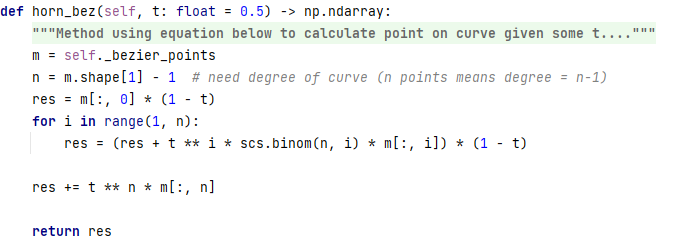
\includegraphics[width=\textwidth]{horner.png}
    \caption{Bézier with Horner Scheme Code}
    \label{fig:my_label}
\end{figure}
Note that \texttt{m} is just a reference to the control polygon for simplicity's sake.

\subsection{Monomial Form of Bézier Curve}
Before we start with the monomial form we need to know how to calculate the derivatives of Bézier curves.
\begin{definition}\label{diff}(Forward Differences and Iterated Forward Differences)
Given some points $b_0, \dots, b_n$ over $\mathbb{R}^2$.
The \textbf{forward difference} is defined as follows:
\[\Delta b_j = b_{j+1} - b_j\]
We can go one step further and define the \textbf{iterative forward differences}:
\[\Delta^r b_i = \sum_{j=0}^r \binom{n}{j} \cdot (-1)^{r-j} \cdot b_{i+j}\]
\end{definition}
These will become handy when we inspect the derivatives and the monomial form.
\newpage
\subsubsection{Derivative of Bézier Curves}
Before we will have a look at the general derivative, let us first examine the first derivative.
\begin{theorem}
For the first \textbf{derivative} we first compute one step of De-Casteljau with $t=1$ and then with an arbitrary $t \in [0,1]$ the next $n-1$ steps.
\[b^\prime(t) = n \cdot \sum_{j=0}^{n-1} \Delta b_j B_j^{n-1}(t)\]
Alternatively we can perform $n-1$ steps of De-Casteljau with respect to some $t \in [0,1]$ and then exactly one step with $t=1$.
\[b^\prime(t) = n \cdot (b_1^{n-1}(t) - b_0^{n-1}(t))\]
\end{theorem}
This leads to an interesting property.
\begin{rem}
The derivative of a Bézier curve is just another Bézier curve, hence the derivative is a byproduct of the De-Casteljau algorithm. Though the De-Casteljau algorithm is not the fastest way of computing a Bézier curve, it is useful whenever we also need the first derivative.
\end{rem}
With the help of \cref{diff} we get a formula for the $r$'th derivative.
\begin{theorem}\label{deriv}
For a Bézier curve described by $b_0, \dots, b_n \in \mathbb{R}^2$ we get that the $r$th derivative is described by
\[\frac{d^r}{dt^r}b^n(t) = \frac{n!}{(n-r)!} \cdot \sum_{j=0}^{n-r} \Delta^r b_j \cdot B_j^{n-r}(t)\]
where $\Delta^r b_j$ is the iterated forward difference of $b_j$ for $j \in \{1, \dots, n\}$.
\end{theorem}
Since we can know easily compute the derivatives we can generate the Taylor series, which is our monomial form, since we are in the polynomial case.
\[x(t) = \sum_{j=0}^n \frac{1}{j!} \cdot x^{(j)}(0) \cdot t^j \]
When we use \cref{deriv} we get:
\newpage
\begin{theorem}
The monomial Form of a Bézier curve with the control points $b_0, \dots b_n \in \mathbb{R}^2$ is decribed by the formula
\[b^n(t) = \sum_{j=0}^n \binom{n}{j} \cdot \Delta^j b_0 \cdot t^j\]
where $\Delta^j b_0$ is the iterated forward difference of $b_0$.
\end{theorem}

\subsubsection{Implementation}
We again use sympy to first calculate the polynom as a symbolic function. This is done by computing the coefficient $\binom{n}{j} \cdot \Delta^j b_0$ and multiplying it with the symbol $t^j$. Finally we use lambdify to fasten up the computation of the function. Hence we end up with a lambda function which takes a $t$ as input and calculates the point. Alternatively one could use the presented Horner scheme by first constructing a list of the coefficients, that has to be done just once, and after that just call the method with the list and every value for $t$.\\

However this form is \textbf{numerical very unstable} and should be avoided whenever possible.

\subsection{Subdivision}
Let us turn our attention to a different approach of computing Bézier curves.
\begin{definition}(Subdivision)
Given $b_0, \dots, b_n \in \mathbb{R}^2$ we run the De-Casteljau algorithm for some given parameter $t \in \mathbb{R}$. After that, we divide our set of points into two. First set is over the interval $[0,t]$, we will denote this points $l_0, \dots, l_n \in \mathbb{R}^2$. The second set is over the interval $[t,1]$, we call these points $r_0, \dots, r_n \in \mathbb{R}^2$. We repeat this procedure for some given amount of $k \in \mathbb{N}$ rounds.
\end{definition}
So subdivision can be seen as an \textbf{approximation} of the curve described by our initial Bézier polygon since we get $2\cdot(n+1)$ points per iteration, which can again be subdivided. Obviously, the more points we evaluate, the better the approximation becomes.
\begin{rem}
After $k \in \mathbb{N}$ rounds of subdivision, one gets $2^k$ Bézier polygons with $n+1$ points each.
\end{rem}
This can easily be seen as per round of subdivision we get two sets of points and we apply subdivision on them in the next step. This leads to a relatively fast approximation of our Bézier curve.
\begin{example}
After $10$ rounds of subdivision with $b_0, \dots, b_5 \in \mathbb{R}^2$ we get $1024$ Bézier polygons each consisting of $6$ points.
\end{example}
Now we will have a look at which points one should pick for the left and right set of points.
\begin{example}
If we look at the cubic example it is also easy to see which points to pick.
\begin{center}
  \begin{tabular}{ l c r r}
  \textcolor{red}{$b_0$} &         \\
  $b_1$ & \textcolor{red}{$b_0^1$} &      \\
  $b_2$ & $b_1^1$ & \textcolor{red}{$b_0^2$}    \\
 \textcolor{blue}{$b_3$} & \textcolor{blue}{$b_2^1$} & \textcolor{blue}{$b_1^2$} & \textcolor{Plum}{$b_0^3$}\\
\end{tabular}
\\
\end{center}

We just take the \textcolor{red}{hypotenuse} and the \textcolor{blue}{bottom line} of the scheme. However the bottom line is taken in \textbf{reversed} order and not from left to right.
\begin{figure}[H]
    \centering
    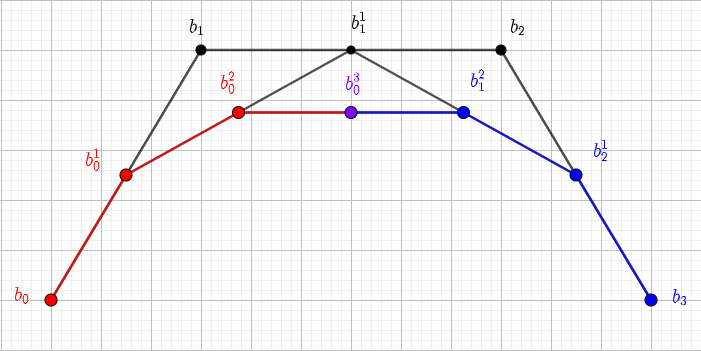
\includegraphics[width=\textwidth]{SubdivisionExamplePic.PNG}
    \caption{Subdivision Example with $t=0,5$}
    \label{fig:my_label}
\end{figure}
In the end we get two new Bézier polygons, which both have four points like the one we had in the beginning, the left one in red with the points $b_0$, $b^1_0$, $b^2_0$ and $b^3_0$ which is shared with the blue Bézier polygon on the right, consisting of $b^3_0$, $b^2_1$, $b^1_2$ and $b_3$.
\end{example}


\subsubsection{Implementation}
We implemented the described procedure in the following way. The \texttt{current} variable represents one column of the triangular scheme we presented. By setting the $ith$ element of \texttt{left} to the fist element of \texttt{current} in every step we always ensure that only elements lying on the hypotenuse are saved in \texttt{left}. The array \texttt{right} works in a quite similar manner but as we want the reverse order we begin at the end of the array and always look at the last element of current which is an element from the bottom line of the scheme. At last in every iteration we call \texttt{de\_casteljau\_one\_step} which returns the next column saved in \texttt{current}. 

\begin{figure}[H]
    \centering
    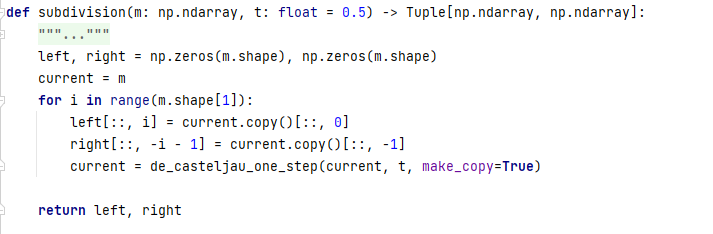
\includegraphics[width=\textwidth]{subdivision.png}
    \caption{Subdivision Code}
    \label{fig:my_label}
\end{figure}

This implmenentation differs a bit; since we double the number of points each time, we have to compute the number of rounds needed for the expected accuracy. We use the following formula:
\[approx\_rounds = \ceil[\bigg]{\log_2 \frac{|\text{points to be calculated}|}{|\text{bezier points}|}}\]
\begin{figure}[H]
    \centering
    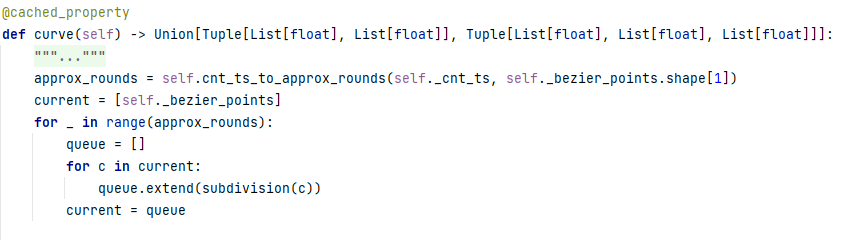
\includegraphics[width=\textwidth]{subdiv_approx_curve.png}
    \caption{Subdivision Code}
    \label{fig:my_label}
\end{figure}
\newpage
With \texttt{approx\_rounds} determined we start a nested loop in which we subdivide for each array contained in \texttt{current}. The resulting \texttt{left} and \texttt{right} are saved in \texttt{queue} which is a temporary storage. At the end we overwrite \texttt{current} with \texttt{queue}. This is done \texttt{approx\_round} times. So for each \texttt{c} in \texttt{current} we get two new arrays. This results in the $2^k$ Bézier polygons where $k$ equals \texttt{approx\_rounds}.

\subsection{Intersection}
In this last section we do not explain another calculation method but instead how one can check whether two Bézier curves intersect thanks to two concepts.

\subsubsection{MinMaxBox}
The MinMaxBox, which is the smallest axis parallel box containing all control points, uses the property of the convex hull. Since all intermediate points $b_i^r$ are computed by a convex barycentric combination of previous points, we never get points outside the convex hull of the $b_i$. Therefore the hole curve described by the control polygon lies within the convex hull. So when we want to perform a fast check of intersection we can construct the MinMaxBox of the two curves, which is just a box containing the control polygon and therefore the curve itself as well. To check if these two boxes intersect can easily be done. If we get a false we can return \texttt{False}. In the other case we have to be more precise. However we can very fast determine if two curves could intersect, which is pretty useful, because we maybe want to check the intersection of multiple curves and with the help of these boxes we can maybe eliminate some curves without taking much effort. 
\subsubsection{Approximate Intersection}
If the two boxes indicate an intersection we have to be more precise, since the intersection of boxes is very coarse. In this case we use subdivision. We split our original curve into sub polygons and check for these ones if their boxes intersect or not, one might call this "divide and conquer". If they do not intersect we can return \texttt{False}. However if they intersect and the areas of the boxes are very small (is defined by a tolerance parameter), we can return \texttt{True}, because our boxes intersect and the box itself can be seen as the part of the curve we are looking at. This is reasonable as we are inherently limited by the floating point precision.\\

In the other cases we just split up again. At the end we check if one of our calls has returned $True$, because then we can say, that the curves intersect with some given tolerance.
\begin{figure}[H]
    \centering
    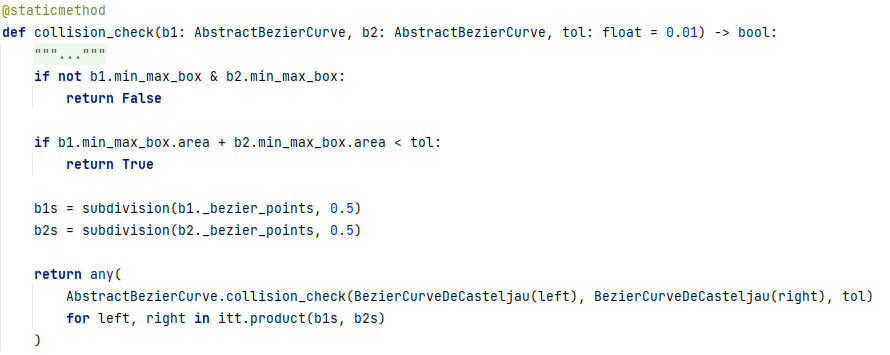
\includegraphics[width=\textwidth]{collision_check.png}
    \caption{Approximate Intersection Code}
    \label{fig:my_label}
\end{figure}

\subsection{Benchmarks}
In order to compare the different algorithms for computing Bézier curves, we ran benchmarks using the same control points.
\subsubsection{Benchmark Configuration}
We used the following configuration:
\begin{itemize}
    \item Dell OptiPlex 5090 Micro
    \item 11th Gen Intel(R) Core(TM) i5-11500T @ 1.50GHz
    \item 1x16 GB non-ECC DDR4 RAM
    \item 256GB NVME M.2 SSD
    \item Ubuntu 20.04.4 LTS (deployed via PXE)
    \item Python 3.8.10
\end{itemize}
The PC was completely idling while running the benchmarks; the idle CPU workload was significantly below 1\%.

\subsubsection{Results}
At first, we compared all viable Bézier curves with each other:
\begin{figure}[H]
    \centering
    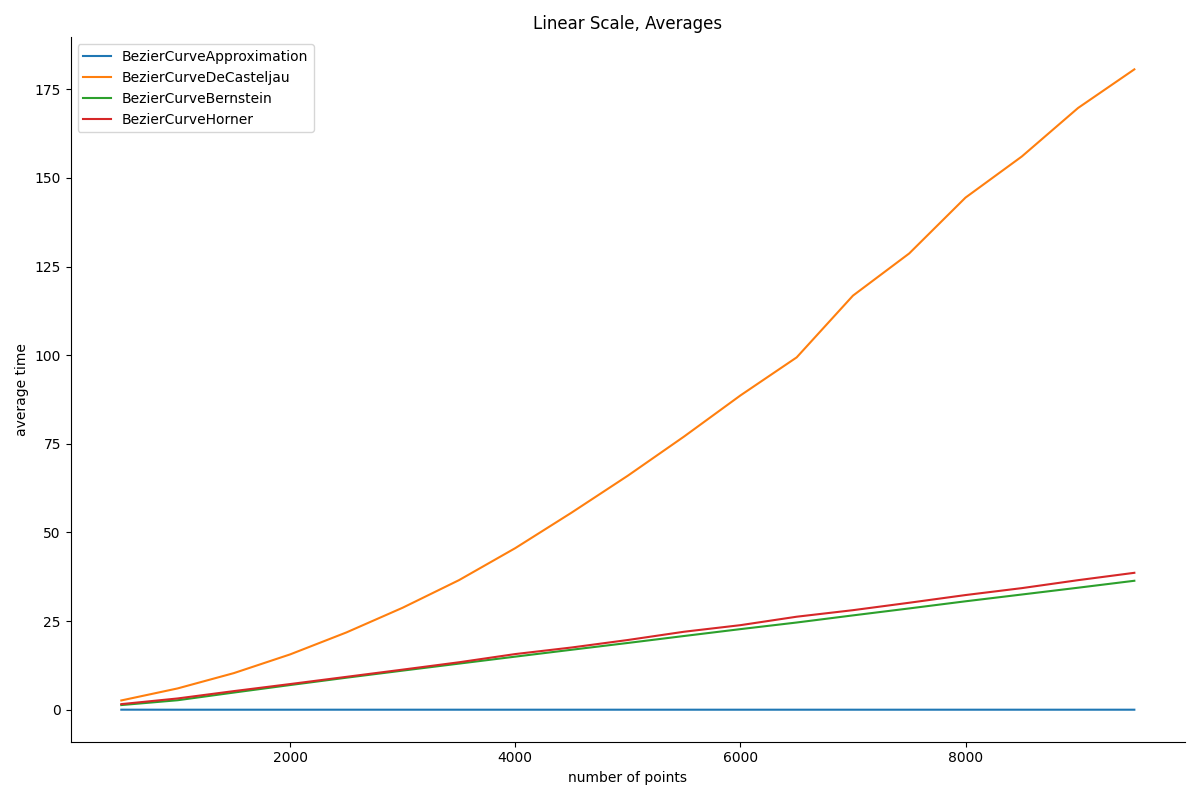
\includegraphics[width=0.9\textwidth]{bezier_lin.png}
    \caption{Average runtime in s}
    \label{fig:my_label}
\end{figure}
To make it more readable, let's look at a logarithmic y-axis:
\begin{figure}[H]
    \centering
    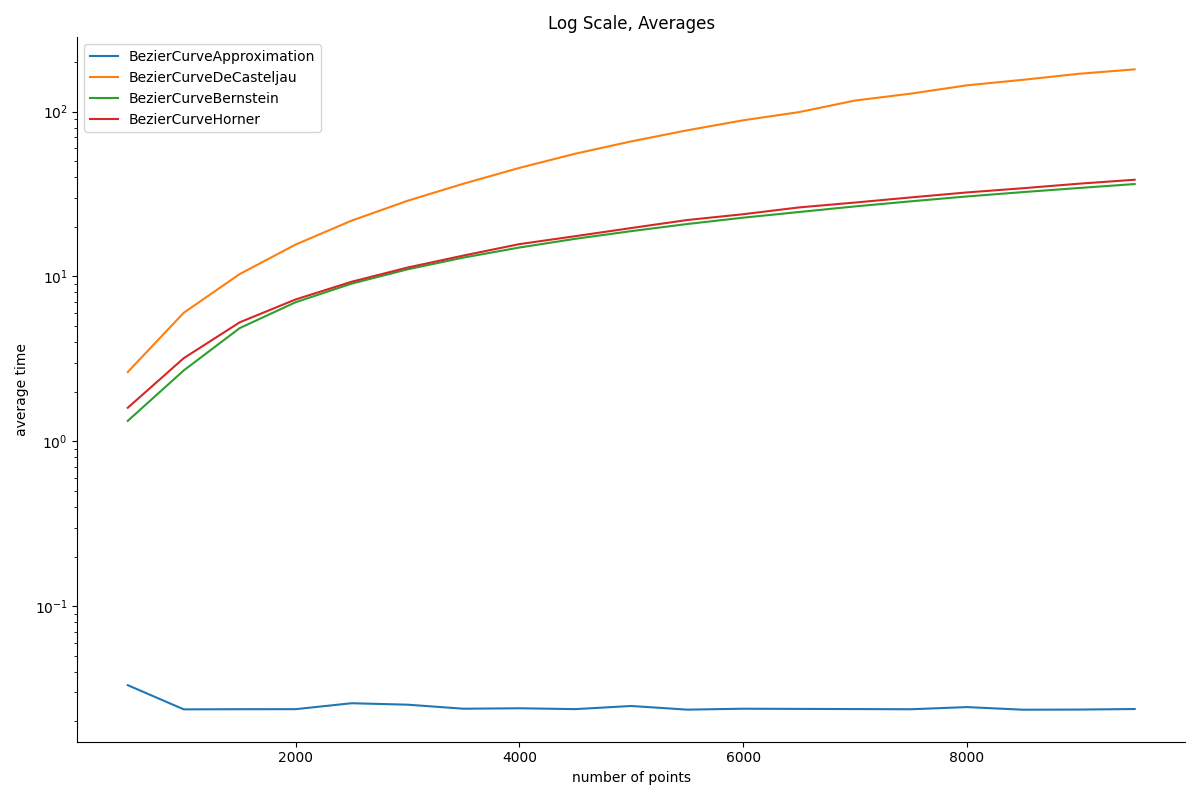
\includegraphics[width=0.9\textwidth]{bezier_log.png}
    \caption{Average runtime in s; logarithmic scale}
    \label{fig:my_label}
\end{figure}
The approximation algorithm seems to have constant runtime. This is not true; as we increase the problem size the real complexity emerges:
\begin{figure}[H]
    \centering
    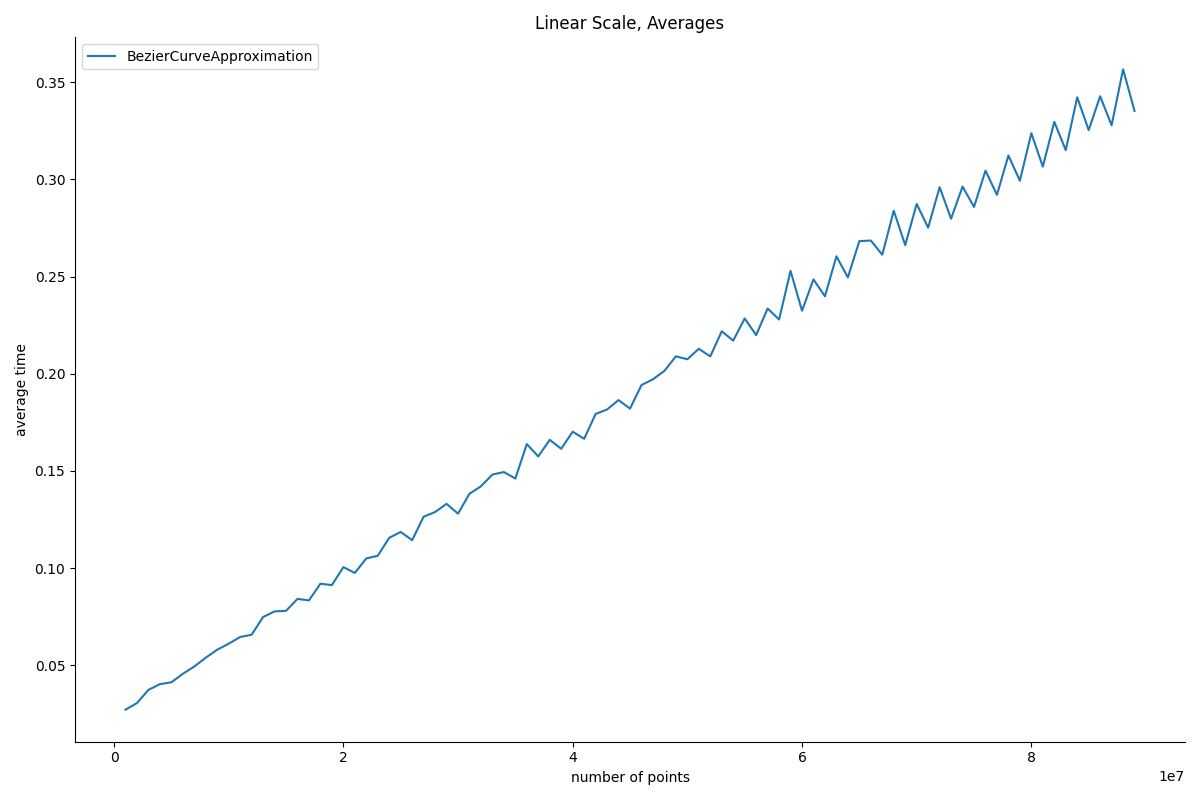
\includegraphics[width=0.9\textwidth]{Approx_lin.png}
    \caption{Average runtime in s}
    \label{fig:my_label}
\end{figure}
Again, in logarithmic scale:
\begin{figure}[H]
    \centering
    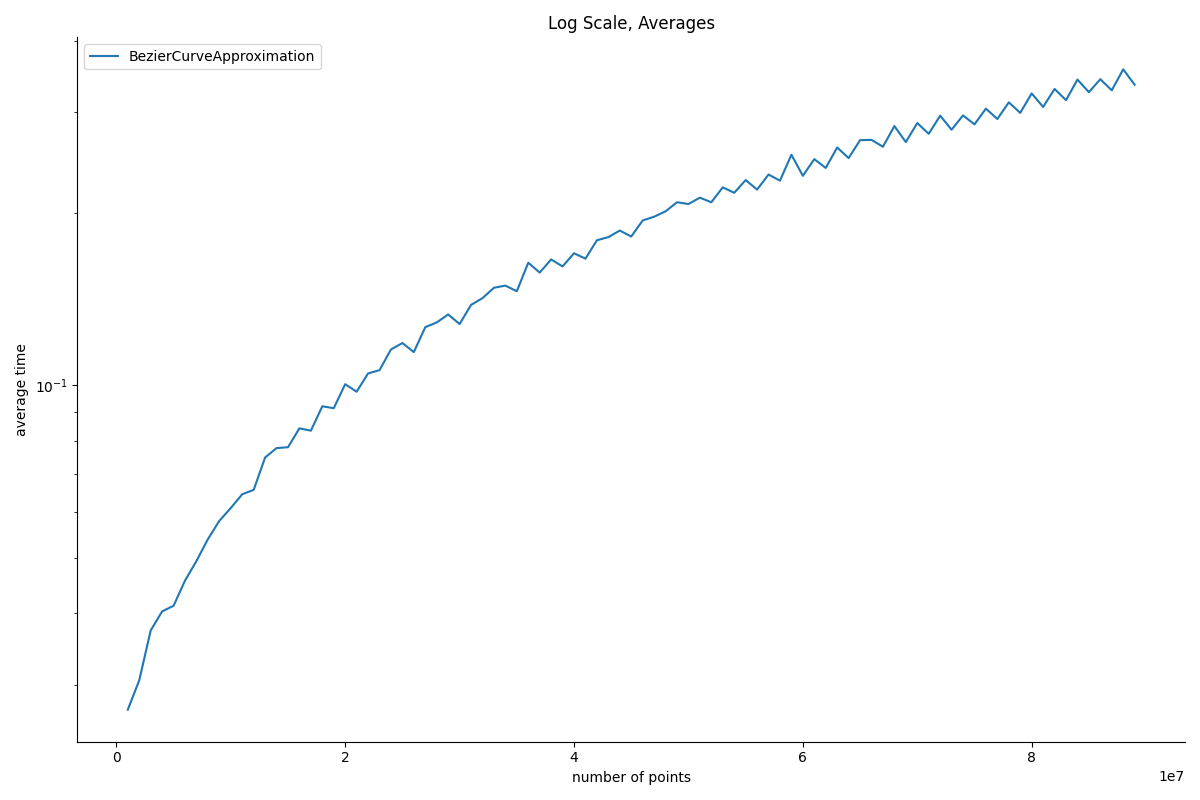
\includegraphics[width=0.9\textwidth]{Approx_log.png}
    \caption{Average runtime in s; logarithmic scale}
    \label{fig:my_label}
\end{figure}
Those are great results, since the computed Bézier curve is, from a visual perspective, basically indistinguishable.
\begin{figure}[H]
\centering
\begin{subfigure}{.5\textwidth}
  \centering
  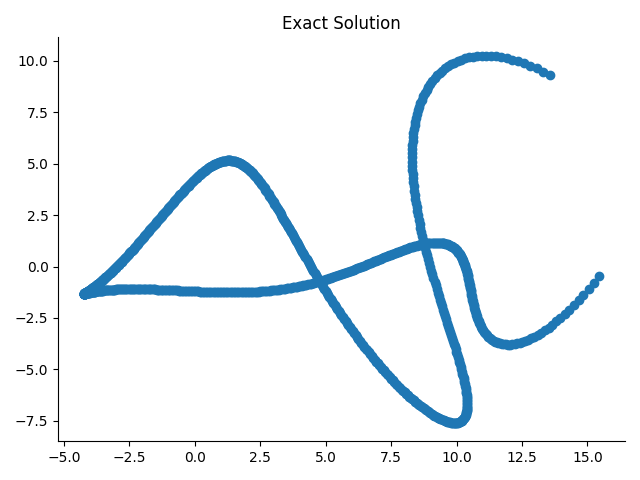
\includegraphics[width=\linewidth]{Comp_Exact.png}
\end{subfigure}%
\begin{subfigure}{.5\textwidth}
  \centering
  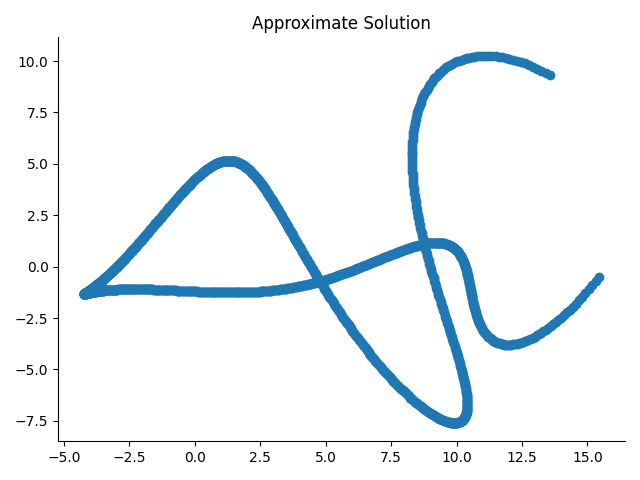
\includegraphics[width=\linewidth]{Comp_Approx.png}
\end{subfigure}
\caption{Both algorithms resulting in the approximately same curve}
\label{fig:test}
\end{figure}

\subsubsection{Problems}
While benchmarking, we encountered two problems:
\begin{enumerate}
    \item As mentioned in the literature \cite{10.5555/501891}, the monomial algorithm is very badly conditioned. Thus, the problem is numerically instable. This would usually not be a problem as Python supports dynamically sized integers. But for large numbers, any floating point values will overflow as they comply with the IEE754 floating point standard. Since $t \in [0,1]$, this can't be avoided.
    \item The Sympy solution does not work for large numbers. This has a rather practical reason. For historical design reasons, Python is designed in such a way that it does not, and will never, support tail call optimization. Therefore the stack space increases linearly with the recursion depth. In order to not get terminated by a segmentation error, Python limits the recursion depth by the variable \texttt{sys.setrecursionlimit}. This also limits the solvable problem size of our Sympy based solution.
\end{enumerate}